\section{Grid 2}
\subsection*{题意}
给定一个 $h$ 行 $w$列的网格,现在位于 $(1,1)$,每次可以向下或右走一格,求有多少种方式(对 $10^9 + 7$ 取模)走到 $(h,w)$。

网格中有 $n$ 个不能经过的障碍,但不会出现在起点和终点。
\begin{center}
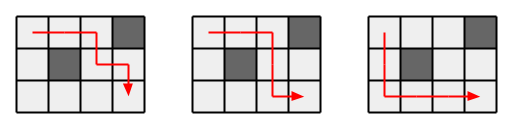
\includegraphics[width=7cm]{./Pics/grid.png}
\end{center}
\subsection*{数据范围}
\begin{itemize}
\item $2 \leq h, w \leq 10^5$
\item $1 \leq n \leq 3000$
\end{itemize}


\subsection*{题解}

(注:由于非此题重点,本题解不包含计算组合数取模的教程,请自行上网搜板子)
本题是 \textit{Grid 1} 的加强版。由于 $h\times w$ 高达 $10^{10}$,无法使用之前的方法。接下来我们来使用常见于\sout{小学奥数}的\textbf{容斥原理}解决这一题。

\paragraph{没有障碍}那么答案就是组合数 $\binom{(h-1)+(w-1)}{h-1}$ ——因为一共要走$(h-1)+(w-1)$步,选择其中的$h-1$步向下。

\paragraph{一个障碍}设障碍格为$(a,b)$,那么答案应该是\uline{总方案数}减去\uline{经过障碍格的不合法方案数},即:
$$
\underbrace{\binom{(h-1)+(w-1)}{h-1}}_{\text{总方案数}} - \underbrace{\binom{(a-1)+(b-1)}{a-1}\binom{(h-a)+(w-b)}{h-a}}_{\text{经过(a,b)的非法方案数}}
$$
\paragraph{两个障碍}设障碍格为$A:(a,b)$和$B:(c,d)$,那么答案等于\uline{总方案数}减去{\uline{经过A的不合法方案数}}减去\uline{经过B的不合法方案数}最后加回被计算了两次的\uline{同时经过A和B的不合法方案数}。 关于最后一部分,这里有两种情况。
\begin{enumerate}
\item 不存在同时经过的路径,如上图所示。那么数量就是 $0$,即答案为 


\begin{align*}
& \binom{(h-1)+(w-1)}{h-1} \\
-& \binom{(a-1)+(b-1)}{a-1}\binom{(h-a)+(w-b)}{h-a}\\
-& \binom{(c-1)+(d-1)}{a-1}\binom{(h-c)+(w-d)}{h-c}\\
\end{align*}

\item 存在同时经过的路径。假设先经过 A 然后经过 B,那么方案数为 
\begin{align*}
& \binom{(h-1)+(w-1)}{h-1} \\
-& \binom{(a-1)+(b-1)}{a-1}\binom{(h-a)+(w-b)}{h-a}\\
-& \binom{(c-1)+(d-1)}{a-1}\binom{(h-c)+(w-d)}{h-c}\\
+& \binom{(a-1)+(b-1)}{a-1}\binom{(c-a)+(d-b)}{c-a}\binom{(h-c)+(w-d)}{h-c}\\
\end{align*}
\end{enumerate}
\paragraph{多个障碍} 总的来说,容斥原理告诉我们,对于障碍的每个子集,如果有奇数个就减去,有偶数个就加上。但 $n$ 个障碍就意味着有 $2^n$ 个子集需要计算,这是无法承受的,我们需要加速。

注意到以下事实:
\begin{enumerate}
\item 如果一个子集中存在一个格子在另一个格子的\textbf{严格}右上方,那么可以直接忽略,因为我们只能向右下方走,无法同时经过。
\item 设障碍的一个子集\textbf{从左上到右下}依次为 $\{(x_1,y_1),(x_2,y_2),\dots,(x_m,y_m) \}$,那么这个子集的贡献为:
$$
(-1)^m\binom{(x_1-1)+(y_1-1)}{x_1-1}
{
\color{Blue}
{
\prod_{i=2}^m \binom{(x_i-x_{i-1})+(y_i-y_{i-1})}{x_i-x_{i-1}}
}
}
\binom{(h-x_m)+(w-y_m)}{h-x_m}
$$
\item 如果把起点和终点也看作的障碍格,那么形式更加简洁: 
$$
(-1)^m\prod_{i=2}^m \binom{(x_i-x_{i-1})+(y_i-y_{i-1})}{x_i-x_{i-1}} 
$$
\end{enumerate}

经过以上铺垫,我们大致可以窥到完整解法的轮廓了。首先把所有障碍(以及起点和终点)按左上到右下的顺序排序。
那么我们设$\texttt{dp}[i][0/1]$表示走到第 $i$ 个格子一共经过了奇数/偶数个障碍。那么转移方程为:
$$
\texttt{dp}[i][0/1] = \sum_{\text{j在i的左上方}} \texttt{dp}[j][1/0] \binom{(x_i-x_j)+(y_i-y_j)}{x_i-x_j}  
$$

初始条件为:
$$
\texttt{dp[(1,1)][1]} = 1
$$

答案为:
$$
\texttt{dp}[(h,w)][0] - \texttt{dp}[(h,w)][1] 
$$

总复杂度是 $O(n^2)$。

\subsection*{核心代码}
\inputminted[linenos,autogobble]{cpp}{./Code/Y.cpp}
\newpage